\documentclass[11pt]{article}
\usepackage[utf8]{inputenc} % LaTeX source encoded as UTF-8
\usepackage[czech]{babel}

\usepackage{graphicx} %graphics files inclusion
\usepackage{amsmath} %advanced maths
\usepackage{amssymb} %additional math symbols
\usepackage{amsfonts}
\usepackage{listings}
\usepackage{hyperref}
\usepackage{color}
\usepackage{graphicx}

\lstset{
	inputencoding=utf8,
	keywords={end,if,for,in,sort, return, and, then},
	keywordstyle=\color{black}\bfseries\em,
}

\begin{document}

\title{1. úloha -- problém batohu}
\author{Ondřej Červenka}
\date{19. 10. 2015}
\maketitle

\section{Specifikace úlohy}

Mějme počet věcí $n \in \mathbb{N}$ a maximální váhu batohu $M \in \mathbb{N}$. \newline Každá věc $i \in \{1, 2, \ldots, n\}$ má určenou váhu $V_i \in \mathbb{N}$ a cenu $C_i \in \mathbb{N}^0$. Úkolem je najít takovou kombinaci věcí, která má co nejvyšší hodnotu a zároveň nepřekračuje maximální váhu batohu $M$.

Problém budeme řešit ve variantě $0/1$, tedy každou věc máme k dispozici pouze jednou. Řešením jsou tedy čísla $\{x_1, x_2, \ldots, x_n\}$, $x_i \in \{0,1\}$ pro která platí $$\sum_{i=1}^n x_iV_i \leq M$$ a zároveň $$\sum_{i=1}^n x_iC_i = max $$ kde $max$ je maximální možná cena.

\section{Řešení}

Úkolem je implementovat algortimus, který nalezne optimální řešení hrubou silou, a algoritmus hledající přibližné řešení pomocí jednoduché heuristiky. Dále pak spočítat chybu heuristiky oproti optimálnímu řešení.

\subsection{Exaktní algoritmus}

Tento algoritmus prohledává všechny kombinace věcí a z nich vybírá řešení s nejvyšší cenou, které zároveň splňuje podmínku maximální váhy batohu. 

Pro $n$ věcí tedy existuje $2^n$ různých kombinací ($x_i$ může mít buď hodnotu $0$ nebo $1$). Algoritmus vždy prohledává všechny kombinace, bez ohledu na to zda překračují maximální váhu $M$ nebo ne. Je tedy datově nezávislý a jeho složitost je $\Theta(2^n)$. 

Algoritmus je rekurzivní, a každé větvení představuje rozhodnutí, zadli přidat nebo nepřidat danou věc do batohu.

\begin{lstlisting}
bruteforce_rec(veci[n], max_vaha, 
	       soucasna_vaha, soucasna_cena, 
               mezivysledek, vysledek,
	       uroven, pridat_vec):
  if (uroven < n - 1) then:
    //pokud nejsme na konci pridej x_i do mezivysledku
    mezivysledek[n+1] = pridat_vec
  end if

  if (uroven < 0) then:
    //pokud je soucasne reseni platne 
    //a lepsi nez dosud nalezene reseni
    if (soucasna_cena > vysledek.cena 
        and soucasna_vaha <= max_vaha) then:
      vysledek.cena = soucasna_cena
      vysledek.vaha = soucasna_vaha
      //vektor x_i popisujici reseni
      vysledek.reseni = mezivysledek
    end if
    return
  end if

  //nepridavat vec do batohu
  bruteforce_rec(veci, max_vaha, 
                 soucasna_vaha, soucasna_cena, 
                 mezivysledek, vysledek, uroven - 1, 0)

  //pridat vec do batohu
  bruteforce_rec(veci, max_vaha, 
                 soucasna_vaha + veci[uroven].vaha,
                 soucasna_cena + veci[uroven].cena,
		 mezivysledek, vysledek, uroven - 1, 1)

\end{lstlisting}

\subsection{Greedy heuristika}

Heuristika hledající přibližné řešení pomocí poměru ceny a váhy $P_i=\frac{C_i}{V_i}$. Algoritmus tedy nejprve seřadí věci podle $P_i$, a poté je postupně vkládá do batohu, dokud není překročena maximální váha.

\begin{lstlisting}
greedy(veci[n], max_vaha):
  vaha = 0 
  cena = 0
  reseni[n] //na zacatku same 0

  //serad veci podle pomeru cena/vaha sestupne
  sort(veci, key=veci.p) 

  for (vec in veci):
    //pokud pridani veci neprekroci maximalni vahu
    if (vaha + vec.v <= max_vaha) then:
      vaha = vaha + vec.v
      cena = cena + vec.c
      //zmen reseni podle indexu veci pred serazenim
      reseni[vec.i] = 1
    end if
  end for

  //vrat nalezenou cenu, vahu
  //a pole popisujici reseni
  return (cena, vaha, reseni)

\end{lstlisting}

Nalezení řešení v seřazeném poli má složitost $\Theta(n)$, asymptotická složitost celého algoritmu tedy závisí na zvoleném způsobu řazení. Při použití quicksortu bude průměrná složitost $O(n \log(n))$.

\section{Výsledky}

\subsection{Podmínky měření}

Algoritmy byly implementovány v C a kompilovány pomocí gcc 5.1.1. Při kompilaci nebyly použity žádné optimalizační přepínače. Program byl zkompilován a spouštěn na operačním systému GNU/Linux (Fedora) 64bit s verzí jádra 4.1.10. Procesor počítače je Intel Core i7-4510U s frekvencí 3.1 GHz.

Vzhledem k proměnlivým časům běhu byly všechny výsledné časy pro heuristický algoritmus získány průměrem z 10 000 běhů algoritmu. Stejným způsobem byly získány časy pro exaktní algoritmus a instance velikosti 4 a 10.

Časy běhu byly získány pomocí funkce $clock()$ z knihovny $time.h$.

\subsection{Výpočetní čas exaktního algoritmu a heuristiky}

\begin{figure}[h!]
	\centering
	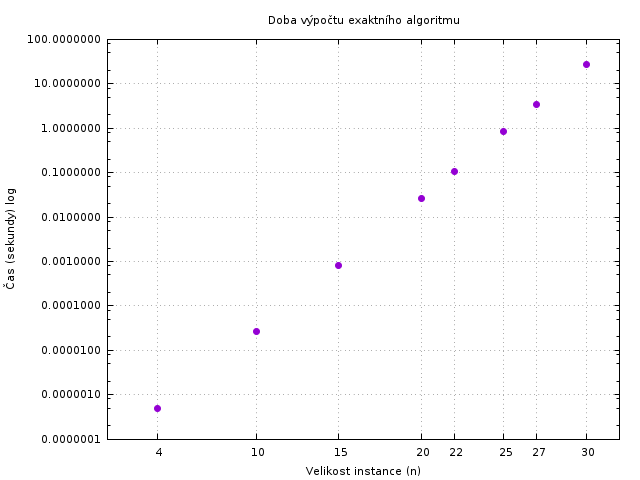
\includegraphics[width=0.8\textwidth]{time_bruteforce.png}
	\caption{Výpočetní časy exaktního algoritmu (v sekundách)}
	\label{fig:time_bruteforce}
\end{figure}

Z grafu (\ref{fig:time_bruteforce}) tedy můžeme vidět, že růst doby běhu výpočtu hrubou silou odpovídá exponenciální funkci (vzhledem k rychlosti růstu je na ose y použito logaritmické měřítko).

\begin{figure}[h!]
	\centering
    	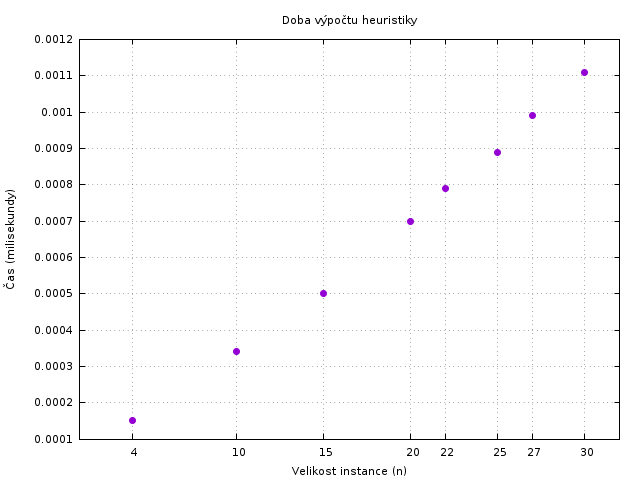
\includegraphics[width=0.8\textwidth]{time_greedy.png}
    	\caption{Výpočetní čas heuristiky (v milisekundách)}
	\label{fig:time_greedy}
\end{figure}

Asymptotická složitost heuristického algoritmu je průměrně $O(n\log(n))$ (quicksort), pro přesnou složitost je ještě třeba připočíst $2n$ pro inicializaci řazeného pole a hledání přibližného řešení. Graf (\ref{fig:time_greedy}) této složitosti odpovídá pouze částečně, což by se dalo vysvětlit velmi krátkou dobou běhu pro všechny instance a omezenou přesností měření.

\subsection{Průměrná a maximální relativní chyba heuristiky}

Chyba heuristiky $\epsilon$ je měřena relativně k optimálnímu řešení, nalezenému pomocí exaktního algoritmu a je počítána pro každou instanci velikosti $n$ zvlášť pomocí vzorce $\epsilon = C(opt) - C(apx) / C(opt)$, kde $C(opt)$ je cena optimálního řešení a $C(apx)$ cena přibližného řešení nalezeného heuristikou.

Grafy zobrazují průměrnou (\ref{fig:avg_error}) a maximální (\ref{fig:max_error}) chybu pro padesát instancí velikost $n$.

Se zvětšujícím se $n$ sice klesá počet řešení nalezených heuristikou, která jsou optimální, ale průměrná chyba je nižší než u $n \leq 10$.

Výkyv maximální chyby u instancí velikosti $27$ je způsoben instnací s 26 předměty s cenou i váhou 12 (jejich poměr ceny a váhy $P_i$ je tedy 1) a jedním předmětem s cenou 349 a váhou 350 (poměr $P_i = 0.9971$).

Tento předmět je tedy vyhodnocen jako nejhorší a do batohu jsou vkládány všechny ostatní předměty. Když tyto předměty dojdou, je výsledná váha i cena 312 a jediný zbývající předmět již překročí maximální váhu batohu, která je 350. Méně výhodný předmět by však batoh zaplnil lépe.

Instance tohoto typu, kdy jsou vkládány poměrově výhodnější předměty, které však nezaplní batoh stejně dobře jako méně výhodné předměty, před\-stavují jeden z problémů této heuristiky. 

Algoritmus by lépe pracoval s variantou problému, kde je od každé věci k dispozici neomezený počet exemplářů, nicméně u výše zmíněné instance by ani to nevedlo k optimálnímu řešení.

\begin{figure}[h!]
	\centering
    	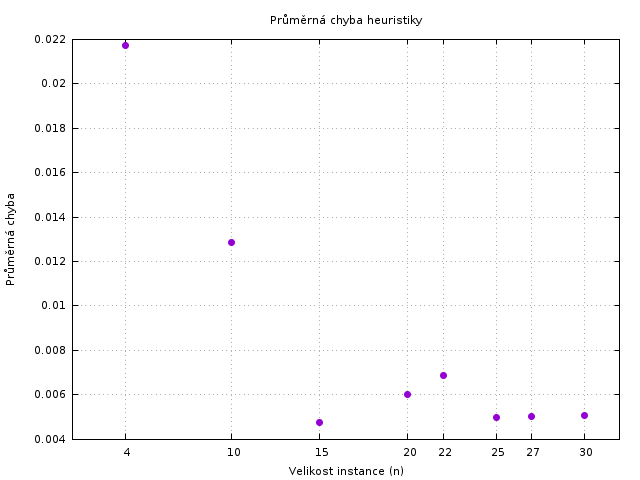
\includegraphics[width=0.8\textwidth]{avg_error.png}
    	\caption{Graf průměrné chyby heuristiky oproti optimálnímu řešení}
	\label{fig:avg_error}
\end{figure}

\begin{figure}[h!]
	\centering
    	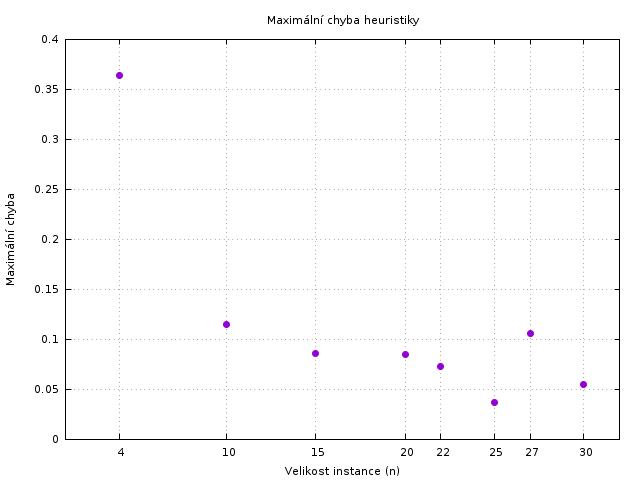
\includegraphics[width=0.8\textwidth]{max_error.png}
    	\caption{Graf maximální chyby heuristiky oproti optimálnímu řešení}
	\label{fig:max_error}
\end{figure}

\section{Závěr}

Ukázalo se tedy, že i velmi jednoduchý heuristický algoritmus dokáže najít řešení blízká optimálním, a to v o několik řádů lepším čase.

Výpočetní doba exaktního algoritmu je únosná pouze pro velmi malé instance ($n \leq 25$), dala by se však vylepšit například ukončením prohledávání, pokud je již jasné, že všechny další kombinace určitě překročí maximální váhu batohu.

\end{document}
